%%%%%%%%%%%%%%%%%%%%%%%%%%%%%%%%%%%%%%%%%%%%%%%%%%%%%%%%%%%%%%%%%%%%%%%
%%%
%%%         【非公式】東京理科大学 創域理工学部 機械航空宇宙工学科
%%%                       卒業論文要旨 テンプレート
%%%
%%%                                  v1.3.0 Yuki MATSUKAWA 01 Feb. 2023
%%%                                  v2.0.0 Yuki MATSUKAWA 14 Dec. 2023
%%%
%%%%%%%%%%%%%%%%%%%%%%%%%%%%%%%%%%%%%%%%%%%%%%%%%%%%%%%%%%%%%%%%%%%%%%%
\documentclass[a4paper,fleqn,dvipdfmx,12pt]{jreport}

%%% abstract style %%%
\usepackage{abstract}
\usepackage{epsf,color}
\usepackage{float}
\usepackage{subfigure}
\usepackage{rotating}
\usepackage{lscape}
\usepackage{bm}
\usepackage{multirow}
\usepackage{multicol}
\pagestyle{empty}


\begin{document}

%%%%%%%%%%%%%%%%%
%%% 日本語要旨 %%%
%%%%%%%%%%%%%%%%%

\begin{center}
\fontsize{16pt}{16pt}\selectfont
{\gtfamily\bfseries ここには卒業論文のタイトルを入れます.\\ 一文字でも間違えたら受理されません.}
\end{center}

\noindent
% 学籍番号,姓,名の間に全角スペース忘れずに
% xx を研究室名に変更
% \hfill は消さない
[xx研究室] \hfill 75***** 姓姓 名名

\vskip\baselineskip
\fontsize{12pt}{16pt}\selectfont
%%% ここから書き始める %%%
アブストラクトアブストラクトアブストラクトアブストラクトアブストラクトアブストラクトアブストラクトアブストラクトアブストラクト
アブストラクトアブストラクトアブストラクトアブストラクトアブストラクトアブストラクトアブストラクトアブストラクトアブストラクト
アブストラクトアブストラクトアブストラクトアブストラクトアブストラクトアブストラクトアブストラクトアブストラクトアブストラクト
アブストラクトアブストラクトアブストラクトアブストラクトアブストラクトアブストラクトアブストラクトアブストラクトアブストラクト
アブストラクトアブストラクトアブストラクトアブストラクトアブストラクトアブストラクトアブストラクトアブストラクトアブストラクト
アブストラクトアブストラクトアブストラクトアブストラクトアブストラクトアブストラクトアブストラクトアブストラクトアブストラクト
アブストラクトアブストラクトアブストラクトアブストラクトアブストラクトアブストラクトアブストラクトアブストラクトアブストラクト.

\fref{fig:abst1}は虎,\fref{fig:abst2}も虎.
アブストラクトアブストラクトアブストラクトアブストラクトアブストラクトアブストラクトアブストラクトアブストラクトアブストラクト
アブストラクトアブストラクトアブストラクトアブストラクトアブストラクトアブストラクトアブストラクトアブストラクトアブストラクト
アブストラクトアブストラクトアブストラクトアブストラクトアブストラクトアブストラクトアブストラクトアブストラクトアブストラクト
アブストラクトアブストラクトアブストラクトアブストラクトアブストラクトアブストラクトアブストラクトアブストラクトアブストラクト
アブストラクトアブストラクトアブストラクトアブストラクトアブストラクトアブストラクトアブストラクトアブストラクトアブストラクト
アブストラクトアブストラクトアブストラクトアブストラクトアブストラクトアブストラクトアブストラクトアブストラクトアブストラクト
アブストラクトアブストラクトアブストラクトアブストラクトアブストラクトアブストラクトアブストラクトアブストラクトアブストラクト
アブストラクトアブストラクトアブストラクトアブストラクトアブストラクトアブストラクトアブストラクトアブストラクトアブストラクト
アブストラクトアブストラクトアブストラクトアブストラクトアブストラクトアブストラクトアブストラクトアブストラクトアブストラクト
アブストラクトアブストラクトアブストラクトアブストラクトアブストラクトアブストラクトアブストラクトアブストラクトアブストラクト
アブストラクトアブストラクトアブストラクトアブストラクトアブストラクトアブストラクトアブストラクトアブストラクトアブストラクト.

\begin{multicols}{2}
   	\begin{figure}[H]
   		\begin{center}
   		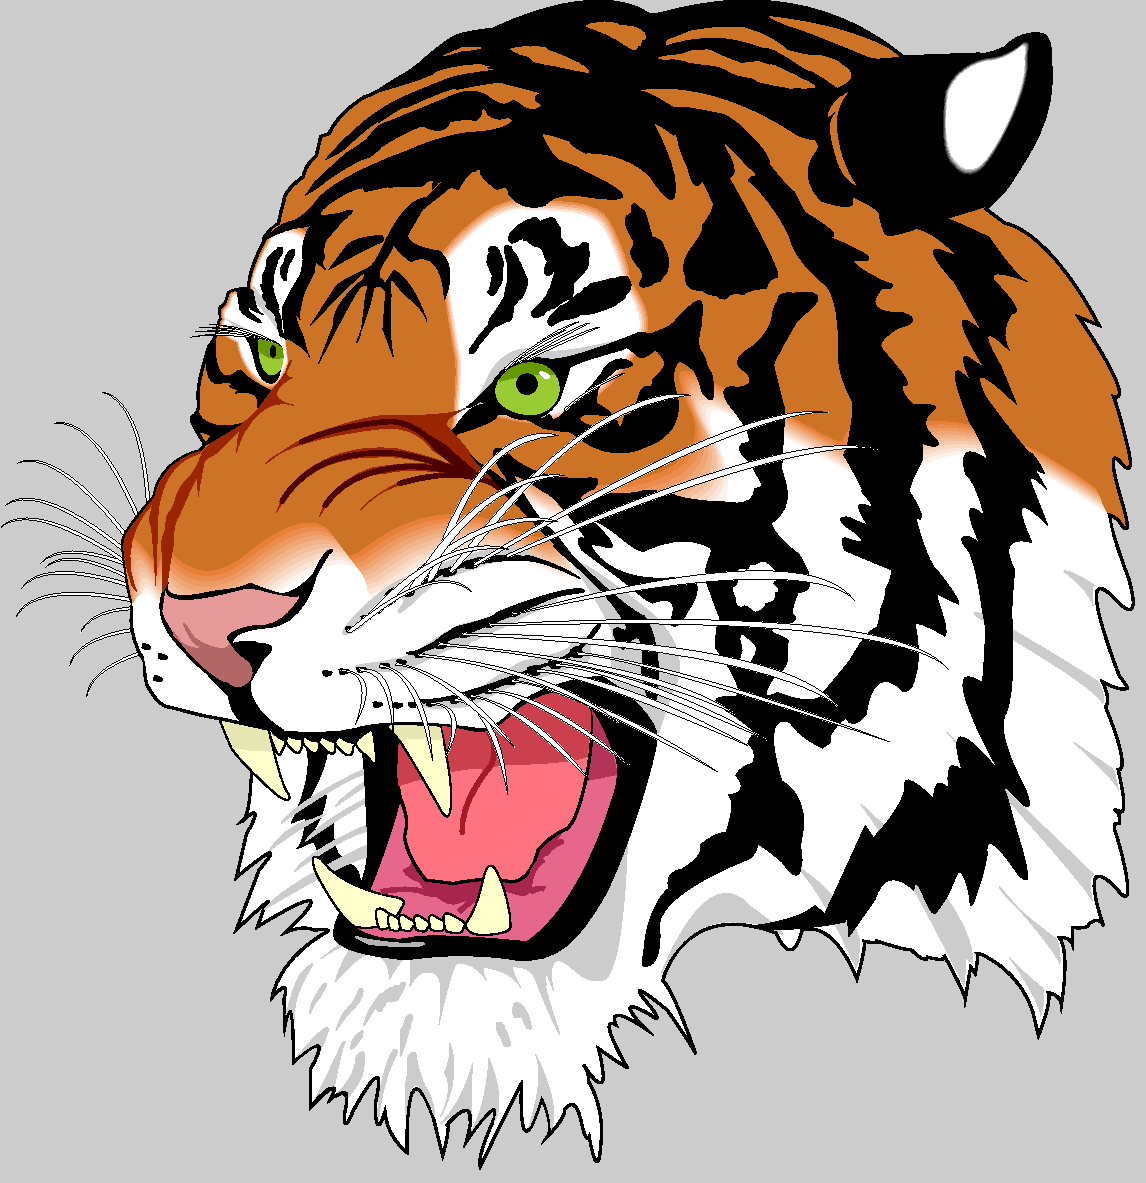
\includegraphics[width=0.6\columnwidth]{tiger.pdf}
   		\caption{Tiger 1.}
   		\label{fig:abst1}
   		\end{center}
   	\end{figure}

   	\begin{figure}[H]
   		\begin{center}
   		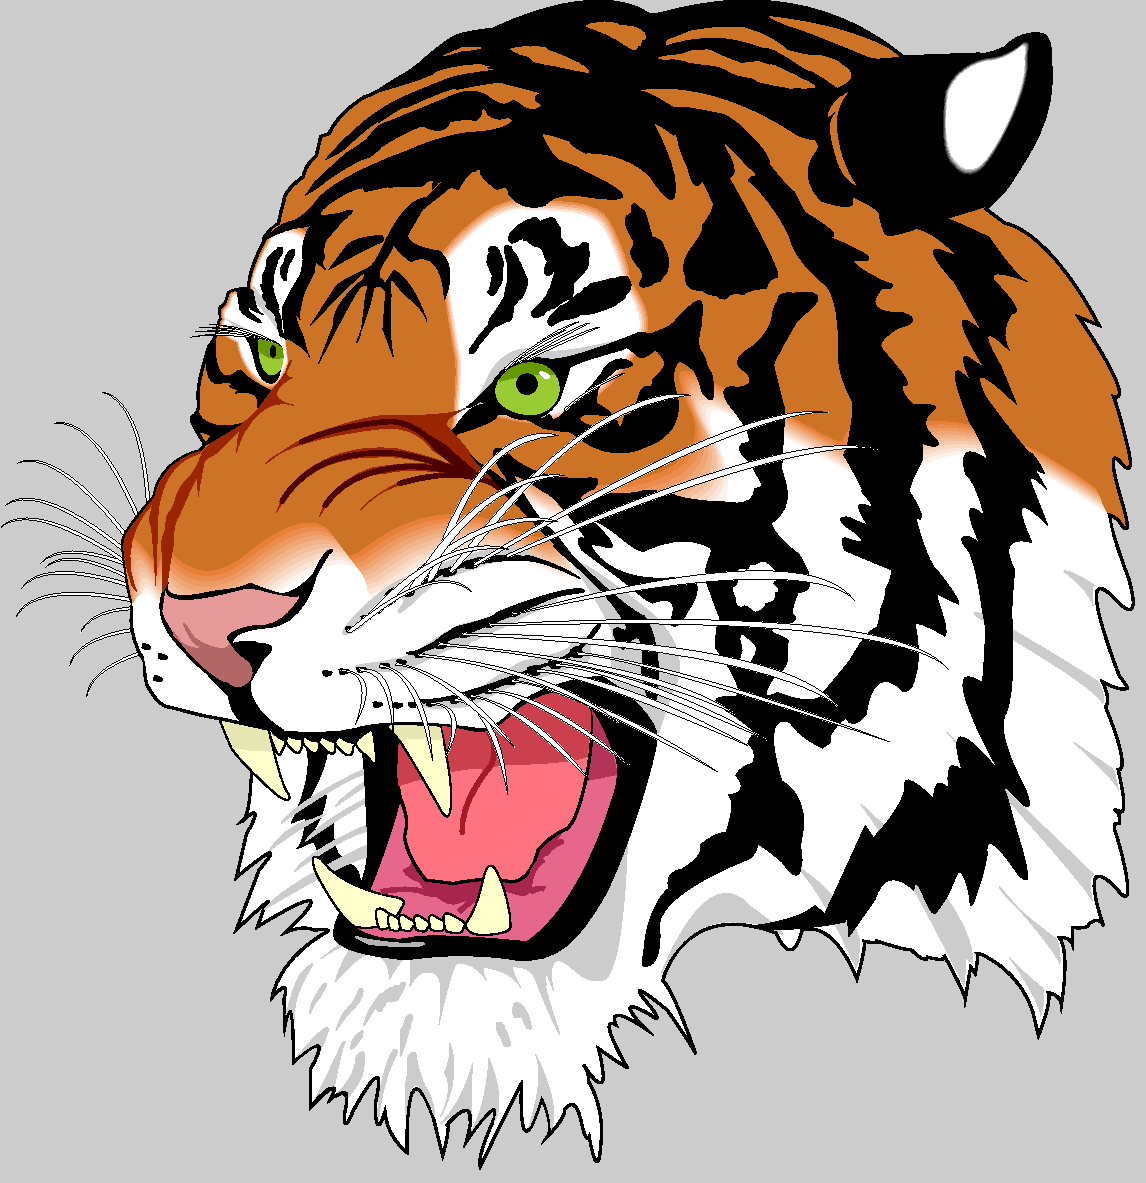
\includegraphics[width=0.6\columnwidth]{tiger.pdf}
   		\caption{Tiger 2.}
   		\label{fig:abst2}
   		\end{center}
   	\end{figure}
\end{multicols}

%%% ここまで %%%

%%% ここで改ページ %%%
\clearpage

%%%%%%%%%%%%%%%%%
%%%% 英語要旨 %%%%
%%%%%%%%%%%%%%%%%

\begin{center}
{\sffamily\bfseries Enter the title of your graduation thesis here. \\ If you make a mistake in even one letter, it will not be accepted.}
\end{center}

\noindent
% 氏名の大文字小文字に注意
% 学籍番号,名,姓の間に半角スペース忘れずに
% xx を研究室名に変更
% \hfill は消さない
[xx Group] \hfill 75***** First FAMILY

\vskip\baselineskip
%%% ここから書き始める %%%
Abstract abstract abstract abstract abstract abstract abstract abstract abstract 
abstract abstract abstract abstract abstract abstract abstract abstract abstract
abstract abstract abstract abstract abstract abstract abstract abstract abstract
abstract abstract abstract abstract abstract abstract abstract abstract abstract
abstract abstract abstract abstract abstract abstract abstract abstract abstract
abstract abstract abstract abstract abstract abstract abstract abstract abstract
abstract abstract abstract abstract abstract abstract abstract abstract abstract
abstract abstract abstract abstract abstract abstract abstract abstract abstract.

%%% ここまで %%%

\end{document}